\documentclass{article}
\usepackage{graphicx}
\usepackage{amsmath}
\usepackage[margin=1.25in]{geometry}
\begin{document}



\section*{Lecture 2}
\begin{itemize}
\item CHDL or HDL is a textual language for designing hardware circuits.
\item Circuits can be specified via a diagram schematic or a textual CHDL.
\item Diagrams are easier for the beginner but not very scalable or useful.
\item CDHLs offer better scalability and support formal methods.
\item Circuits are very similar to functions. Black box, internal computation, produce outputs.
\item Give circuits a name in Hydra. This type of 'black box' definition is similar to abstraction in imperative programming languages.
\item Multiplexor in primitives: mux1 c a b = or2 (and2 (inv c) a) (and2 c b).
\item Think of the multiplexor order ar counting from 0 to highest ed mux2 (0,1) p q r s = q (second value).
\item Demultiplexors take an control input and a data input and produce 2 outputs. The control selects which output to put the data on.
\item Demux2 and Mux2 can be built by combining demux1s or mux1s
\item Tuples used where there is no logical grouping and indexing doesn't make sense.
\item Words used when there is a logical sense of numbering and ordering.
\item Words of Tuples and Tuples or Words are allowed.
\end{itemize}



\section*{Lecture 3}
\begin{itemize}
\item No feedback loops in combinational logic.
\item Make sure that inputs and outputs are known BEFORE implementation.
\item Efficiency is tied in with a circuits cost model. Not necessarily the number of components.
\item It is generally better to come up with a better algorithm.
\item In VLSI regularity is better than random optimization.
\begin{enumerate}
\item Synthesis from truth table.
\item Synthesis from algebraic logic
\item `'Sum of cases" technique.
\item Conditionals and cases.
\item Using encodings.
\item Defining building blocks
\item Standard patterns
\end{enumerate}
\item `'Sum of cases" technique is a way of truth table synthesis. (mapping inputs to outputs)
\item Nested multiplexors are used for conditionals and cases.
\item Cases correspond to $2^k$ cases given a k-bit opcode. Use demultiplexors in these circumstances.
\item Half adder - A sum and a carry. Full adder a 2 bit sum and a carry.
\item Ripple adders are combinations of the 'full adder' building block
\end{itemize}
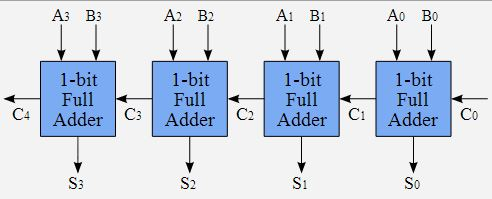
\includegraphics[width=\linewidth]{rippleadd}
\begin{itemize}
\item Efficiency should always be done in reference to cost model.
\item Optimization only plays a part later, it should not interfere with synthesis or it could become counterproductive.
\item Cost models place a cost on a circuit. The best circuit is the one with the lowest cost.
\item Examples of cost models include number of components (not useful nowadays as we have integrated circuits) and path depth (for combinational circuits).
\item For k inputs. There are $2^k$ lines in its truth table and $2^{(2^k)}$ boolean functions of k inputs.
\item General logic gates (LUT). Important in reconfigurable circuits. p = lut2 (a,b,c,d) x y
\item Gate delay is the time it takes for a signal to become valid once it has reached the gate.
\item Difference between invalidity and incorrectness.
\item For each signal x in the circuit, the time at which x becomes stable is called t(x). This is the path depth of x
\item Inputs to x are denoted a I(x).
\item Gate delay of a gate = gate delay of previous gates and the gates own delay. \[ t(x) = d + \underset{y \in I(x)}{\text{max } t(y)} \]
\item Critical path depth is the maximum path depth of all of its outputs. This can be used to determine the 'speed' of the circuit.

\end{itemize}


\section*{Lecture 4}
\begin{itemize}
\item Hazards, incorrect output based on varying gate delays (ie and2 x (inv x) results in a 1 value while (inv x) suffers gate delay).
\item A sequential circuit may have flip flops and feedback loops.
\item Sequential circuits perform computations through time.
\item Flip-flip is basic memory (hydra def - dff :: Clocked a $\rightarrow$ a $\rightarrow$ a)
\item Clocked used a Bool is simply not rich enough.
\item Real systems have a reset mechanism to put flip-flips into a valid state.
\item System must ensure a valid flip-flip value (no mid-voltages).
\item Flip-flops update on clock tick. Output continuous but only updates when clock pulses 1.
\item Abstract clock and Physical clock differences. Abstract cannot exist in real life. Components treat a 0 to 1 transition as a tick.
\item Synchronous model is used to prvent hazards. It boasts simple behavior and satisfies some constraints.
\item Synchronous if:
\begin{enumerate}
\item Contains logic gates and flip flops.
\item Every flip flop is connected to a global clock.
\item Every clock tick reaches each flip flop at the same time.
\item Each feedback loop goes via a flip flop.
\item Inputs to a circuit remain stable during a clock cycle.
\end{enumerate}
\item The restrictions on this mean that you cannot do combinational logic on clock input, you cannot introduce state via combinational feedback loops, and the circuit may malfunction if inputs are not stable for long enough.
\item State can be created by using flip flops or feedback loops in combinational logic (difficult to reason).
\item A synchronous circuit is a sequential circuit that behaves like a finite state automation.
\item Synchronous trade off. Restricted design chouce but much easier to reason the circuit.
\item Clock is an implicit input (as all dffs have the same clock ALWAYS).
\item Clock tick is a point in time. Clock cycle is an interval.
\item Clock skew is when a clock tick does not reach flip flops at the same time (such as in a fanout or if there are longer wires etc). 
\item The floor plan of the clock is normally laid out well in advance. See example H-tree. Known as the clock distribution.
\end{itemize}
\begin{center}
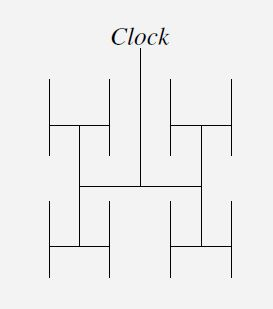
\includegraphics[width=0.5\linewidth]{hlayout}
\end{center}
\begin{itemize}
\item Circuits can have 'global' state in the synchronous model (values of all flip flops).
\item Circuit behaves as a single finite state automation.
\item Clock removes concern for intermediate values, hazards and gate delays (as they are all dealt with in the synchronous model).
\item reg1 component like a dff but with option ld signal that loads/ignores input value after clock tick accordingly.
\item reg1 works by multiplexing the input to a dff depending on the value of ld (obviously involves a feedback loop).
\end{itemize}


\section*{Lecture 5}
\begin{itemize}
\item list structure for words similar to haskell notation ie. (x:xs) = [a,b,c,d,e], x = a and b = [b,c,d,e]
\item equally the ++, !! and length operators can be used like in haskell.
\item field w i k takes the value of w starting at position i for k elements.
\item The type of a circuit describes its input. Such as how it's represented, how many inputs/outputs it takes/produces, parameter size and building blocks (if any).
\item You may use circuit generators to save making every component by hand. Eg. rippleAdd, a generic n-bit ripple adder that works for any word size.
\item This is not software to do the operation, it is still a real circuit.
\item Hydra has 4 'times'
\begin{enumerate}
\item Model Transformation Time
\item Circuit Generation Time
\item Simulator Compilation Time
\item Runtime
\end{enumerate}
\item Always use type a rather than Bool, its a hydra thing...
\item bitslice2 can be used so that [a] $\rightarrow$ [a] $\rightarrow$ [(a,a)]
\item mux1w is like a multiplexor but outputs words rather than single bits.
\item general n-bit reg an wlatch (wlatch doesn't take a load signal).
\item Modern RISC and CISC architectures use an indexed set of registers R0, R1, R2 etc which are implemented in a circuit called the register file.
\item Memory locations are usually bytes while registers contain words. Registers are few in comparison to memory (but much faster).
\item A dual-port register file provides separate input from output. Some register files have three ports (one in and 2 out).
\item How to handle address inputs. A tree of multiplexors and demultiplexors is needed for the addresses.
\item Look over register file recursive definitions.
\end{itemize}



\section*{Lecture 6}
\begin{itemize}
\item A test bench takes readable input and produces readable output. It converts to and from the actual signals and formats the output.
\item Lots of hydra test bench definitions. 'getbit', 'getbin' and 'gettc'
\item Additional hydra functions 'fanout', 'shl', 'bitslice2', 'orw'
\item An ALU is a combinational circuit. It is typically an adder with augmented functions to support other functions (eg bit shifting, subtraction, incrementing).
\item The critical path of the ALU should be very small.
\item Multiplication, division etc are performed over a series of clock ticks (by using sequential algorithms).
\item Sequential functions may operate as a machine language program, using normal processing registers or using a dedicated sequential circuit with its own registers (functional unit).
\item A functional unit is a sequential black box circuit with its own specific registers to perform a task like multiplication. It receives an input start and outputs an output signal 'ready'.
\item By using a functional unit (which is sequential), we can accept it may take a few clock cycles which means the global clock doesn't have to be slowed down.
\item If it were done by combinational logic the path depth would be so great the clock speed would have to be slowed down.
\item Use the shift and add algorithm to do multiplication. The inputs to x*y would be x y and start, the outputs would the be result and ready.

\end{itemize}



\section*{Lecture 7}
\begin{itemize}
\item Number of patterns in combinational logic; sum of cases, truth tables, fold, scan, map.
\item Design patterns are higher order functions. They take one or more circuit specifications as parameters.
\item The pattern defines how to connect up these given circuits in a regular pattern.
\item Pattern definition similar to ordinary circuit specification except that: It uses recursion to decompose groups of signals, it uses abstract circuits, rather than specific circuits, its type may include building block circuits.
\item map, map2, mapn used as in haskell.
\item fold as well. and2/or2 operate by using left folds.
\item ascanr is like fold but returns a list (including all intermediate values

\end{itemize}



\section*{Lecture 8}
\begin{itemize}
\item FSA (finite state automation) has a set of states, a stream of inputs (and state conversion function). It is used to recognize if the grammar of an input is correct.
\item FSAs need to be more general for practical applications. For example the new state transition function could produce a new output as well as defining a new state to enter.
\item In an unencoded representation you could use a dff for each state. If exactly one flip flop contains a 1 then it is in that state.
\item In an unencoded representation the no. of states = no. state flip flops.
\item In an encoded representation, each possible state is represented by a unique binary number held in a register.
\item In an encoded representation, $\text{no. of flip-flips} = \log_{2}(\text{no. of states})$
\item For the shift and add algorithm we must distinguish between what to put in the registers when start = 1 AND what to put in the registers when start $\neq$ 1 but a multiplication is still taking place.
\item When start = 1 x \& rx are both k bits, y i k bits, ry is 2k bits (it needs padding) and prod is 2k bits. rx and ry are set to the inputs on signals x \& y and prod is set to 0.
\item rx and ry are shifted right and left accordingly so that the algorithm is always examining the same bits.

\end{itemize}



\section*{Lecture 9}
\begin{itemize}
\item Sigma 16 is a 16-bit RISC style architecture. No bytes/words. Everything is 16-bit. 16 registers. Based on a simplified version of MIPS.
\item RRR format (two operands in the register file. The result goes into a register)
\item RX format (one operand is a register, the other is a memory address).
\item Memory addresses are constants, they are the combination of the displacement and the index/base.
\item RRR takes 4 inputs. The opcode op, destination d, and source addresses sa \& sb.
\item RX takes 4 inputs. The RX opcode (MUST be f), a destination register d, an index register sa and the secondary opcode sb.
\item RRR (one word) RX (two words, 4 4 bit fields and a 16-bit displacement).
\item Instructions can often be implemented without a feedback loop.
\end{itemize}
\begin{center}
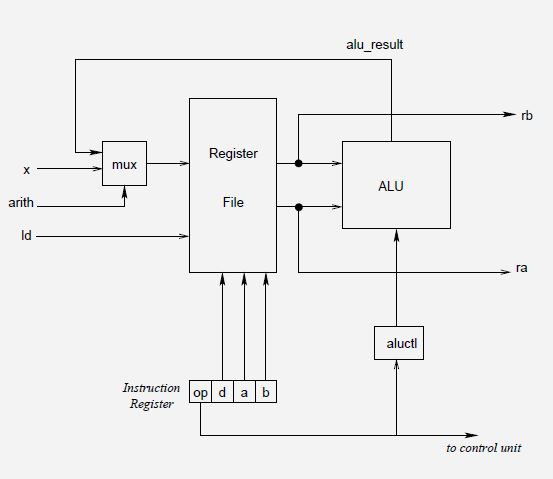
\includegraphics[width=\linewidth]{rtm}
\end{center}
\begin{itemize}
\item The datapath contains the combinational logic for calculations.
\item The control generates all of the control signals needed for the datapath
\item Similar design complexities, the datapath focuses more on structure whereas the control focuses on behavior.
\item Different design techniques (datapath designed directly as a circuit, control as an algorithm). The separation helps clarify timing.
\item Design of the datapath (all the logic and registers needed for calculations) will logically create a set of control signals that operate it.
\item There is a naming convention for control signals. ctl, subsystem, specific. Eg ctl\_rf\_ld.
\item The datapath contains registers, computational systems and interconnections.
\item It has two inputs, the control signals and a data word (from either memory system or the DMA input controller).
\item It outputs the bus to memory an I/O (it also outputs the states of the registers).
\item The datapath can be broken down into further subsystems (registers, ALU, busses etc).
\item Introduce an instruction register and program counter. For RX instructions an adr register is needed for the second word
\end{itemize}


\section*{Lecture 10}
\begin{itemize}
\item adr, pc and ir needed in the datapath to keep track of program execution. ALU needed to perform arithmetic.
\item The datapath contains the processor's registers. 
\item Aim to implement instruction set by an algorithm that uses the registers as temporary variables.
\item Computations on registers are performed via combination logic in the datapath.
\item registers and multiplexors have load control/control signals. The overall behavior is determined by these control signals.
\item many datapath subsystems take control input. The right values must be place on all control signals to make the datapath do something useful.
\item To perform an operation control signals and data inputs must be set (memdat coming from the system memory bus). Outputs will appear at the next clock cycle.
\item almost always will the ir need to be set and the pc incremented. ir:= mem[pc], pc := pc + 1 (the comma denotes that they occur in parallel).
\item **Perhaps look at example operations** Lecture very practical based.
\end{itemize}


\section*{Lecture 11}
\begin{itemize}
\item General behavior of the datapath is defined by the control algorithm. Which is described with high level statements such as ir := mem[pc].
\item A circuit must be designed that will generate the correct control signals to be useful.
\item High level control algorithm $\rightarrow$ determine which signals must be asserted to achieve each statement $\rightarrow$ synthesized control circuit to set the control signals.
\item **Learn some examples of high level control RRR and RX functions**
\item Imperative languages have:
\begin{itemize}
\item Computational Statements - assignments etc.
\item Control Structures - concerned with what and when (eg if-then-else, while loops etc).
\end{itemize}
\item A control language needs:
\begin{itemize}
\item Computational Statement - which control signals should be set. (eg. Assert - which control signals are on/off).
\item Control Structures (similar to those in imperative languages).
\end{itemize}
\item Straight-line control mode. A sequence of assert statements dictate what the control signals will be for a number of clock cycles.
\item Statements can also be given names such as state\_1 : Assert [ctl\_a, ctl\_b, ctl\_c]. Meaning state state\_1 is synonymous with ctl\_a,b,c all being set to 1 and all others being set to 0.
\item Control structures must also be considered, the most important are:
\begin{itemize}
\item Repeat Forever
\item It-Then-Else
\item Case (multi-way conditional)
\item While
\end{itemize}
\item Sequences of statements can be embedded in a 'block' (between begin and end). While they still require several clock cycles to execute, it can be convenient for grouping.
\item Almost every control structure REQUIRES an infinite loop, otherwise the datapath would stop doing things as the control would terminate giving it control signals.
\item fairly obvious case and if-then-else notation.
\item From high level to low level. high level control algorithm can be used an an emulator (executes machine language at register transfer level).
\item Aim is to translate this high level control algorithm into a circuit
\begin{enumerate}
\item For each step, determine the control signals that must be set during a clock cycle.
\item Develop a circuit that generates those signals.
\end{enumerate}
\item **More examples to look at**
\item Specify control algorithm, synthesize a control circuit from the algorithm, when changes are needed, modify the algorithm and re-synthesize. (part of synthesis of control).
\item Synthesis techniques. The delay element method. Simple, flexible and efficient but complex and irregular wiring.
\item Done by having 1 flip-flop per state. At any time only 1 flip-flip contains 1. If a flip-flip is in state 1 it means that corresponding statement is being executed.

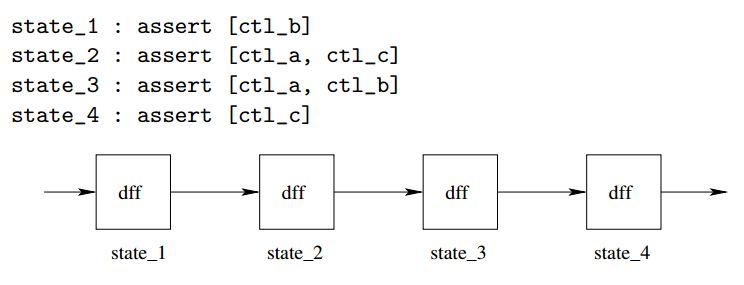
\includegraphics[width=\linewidth]{sdff}[h]
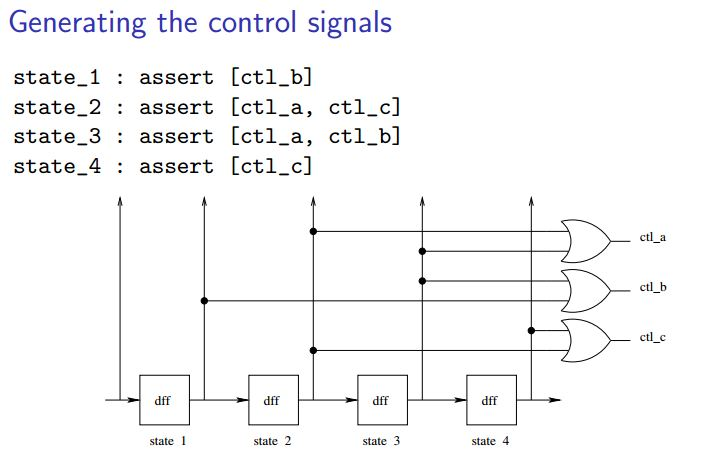
\includegraphics[width=\linewidth]{gcs}[h]

\item **Again more examples**
\end{itemize}

\section*{Lecture 12}
\begin{itemize}
\item M1 is the first version of a circuit that implements the Sigma16 instruction set architecture. 2 ways to run Sigma16 programs, via an emulator or a circuit simulator on the M1 circuit.
\item Several approaches to implement I/O in real systems. 
\begin{itemize}
\item I/O instructions, read and write. Only in early computers. V. Slow.
\item Start I/O instruction. Device generates interrupt when ready.
\item Dedicated I/O processor, running concurrently with CPU. Used in many supercomputers.
\item Direct Memory Access. I/O implemented by stores and fetches at 'magic' memory addresses.
\end{itemize}
\item M1 doesn't support general I/O. It has a special facility for loading a machine language program into memory (DMA).
\item DMA = 1, one word is place in memory each clock cycle, simulation driver is given a list of words and puts it in memory (one per cycle).
\item When finished the simulation driver puts 1 on reset of one cycle which starts the control algorithm.
\item **DMA examples**
\item Software tools include: Assembler, Emulator, Circuit, Circuit Simulator, Simulation Driver.
\item Two main environments higher level (emulation) and lower level (circuit simulation).
\item Higher level: a suite of tools (with GUI) including assembly and emulator. Done in Hydra. Good for assembling programs, referencing behavior and long executions.
\item Lower level: Compile a Sigma16 program with M1 circuit, M1 simulation driver and Hydra library. Produces a standalone application that executes on the Sigma16 program by running it on the circuit.
\item **Assessed Exercise Details and ArrayMax.hs M1 program**
\item M1 and subsystems output internal registers and signals so they can be observed during execution.
\item Simulation driver is different from the ones seen so far as it supports DMA, input is a program (not raw signals) and detects significant output events.
\item **More Examples**
\item IMPORTANT NOTE. The last 2/3 lectures have been rife with examples. These notes may not be sufficient to understand (and more importantly apply) the content described.

\end{itemize}

\section*{Lecture 13}
\begin{itemize}
\item Latency is the time required for an operation. There is memory, instruction and communication latency.
\item Throughput is the amount of work performed per unit of time (eg. memory accesses per second).
\item For overall performance throughput is important.
\item For (re)solving bottlenecks, latency is often important.
\item Amdahl's law observes that the total speed up of the system may be less than the speed up of a part of the system depending on how much time is spend in said part of the system.
\item Example of Amdahl's law. If part A of a system can be sped up from 30s to 15s and is 30\% of the system process (the other part takes 70s) then the increase is 85s/100s which is 1.17 overall speed up factor.
\item Moore's law observes manufacturing trends. It states that the number of transistors per chip will double every two years (or some other number of years). 
\item Moore's law is based on the fact that integrated circuit fabrication technology makes gradual improvements which allows more components to be placed on chips.
\item Moore's law is not about speed. It is about chip density. The only way to increase speed now is to add more processing cores to a chip.
\item Performance should only really be measured in terms of its 'wall clock' time to run a piece of software.

\[  T = \text{ni} \cdot \text{cpi} \cdot \text{spc} \]
\[or\]
\[ T = \frac{\text{ni} \cdot \text{cpi}}{\text{cps}} \]

\item Where T = execution time in seconds, ni = no. instructions in order to execute the program, cpi = average no. clock cycles per instruction, spc = seconds per clock cycle, cps = cycles per second.
\item Reducing one of these factors does not necessarily reduce T.
\item In practice, the critical path will be the path from a register in a register file, through the ALU and back to the register file.
\item The M1 control algorithm will place whatever value is on the memory bus into the destination register. Even if the value is incorrect (for instance if it takes several clock cycles to compute).
\item More sophisticated solutions include using pipelining stages, interleaved memory and superscalar memory.
\item The M1 circuit has no interrupts, memory protection or virtual memory. No concurrency. Long-running instructions must execute until completion while the rest of the processor waits.
\item Pipelining is the application of parallelism to the steps in executing an instruction.
\item General approaches to improving speed include: improving clock speed (reduce critical path), reduce no. clock cycles (pipelining and superscalar parallelism), improve speed of memory (parallelism by interleaved memory, explot locality).
\item The basic application of pipelining is to execute steams of instructions.
\item 'overlapping the steps in consecutinve multiplications'.
\item In multiplication, it is the idea of unrolling iterations.
\item The functional unit has one register for each of the the variables, each clock cycle the new variable overwrites the old variable. This is modified to make a sequence of register triples, each cycle the variables move from one set of registers to the next.
\item 2 related techniques for improving speed. RETIMING - introduce extra registers to break up long paths through combinational logic. Allows for faster clock.
\item PIPELINING - a stream of inputs goes through a sequence of stages. Introduce parallel execution among the stages. Same kind of speed up as an assembly line in manufacturing.
\item The idea of retiming is to find the critical path and break it into smaller paths with registers in between. It will not take several clock cycles to perform the critical path operation but the clock can now be made faster.
\item The critical operation becomes slower due to the safety factor, whereas non-critical operations will benefit speed up.
\end{itemize}

\section*{Lecture 14 (Incomplete)}
\begin{itemize}
\item More stages in pipelining for RX instructions. (fetch second word of instruction, calculate ea, perform memory access).
\item All instructions have to go through the same sequence of stages, so pipeline must have enough stages for the worst case.
\item Conflicts caused by sequencing in pipelining are called hazards. Some can be circumvented by introducing more circuits, some require stalling the pipeline, so we get sequential execution for a brief time.
\item Important to maintain correct behavior.
\item To avoid structural hazards, we separate memories for instructions and data.
\item Data hazards occur when the 'wrong' value is accessed. Similar to critical sections in imperative programming.
\item There are 2 main classifications:
\begin{enumerate}
\item Read After Write
\item Write After Read
\item Write After Write
\item Intuitively, there is no hazard invoked from a Read After Read
\end{enumerate}
\item To detect hazards, we must make a complete list of hazards and introduce combinational logic to check them all. It is essential to find ALL the potential hazards.
\item To detect a read after write hazard:
\[ \text{raw} = (ir1\text{\_sa} = ir3\text{\_d}) \lor (ir\text{\_sb} = ir3\text{\_d}) \]
\item To handle data hazards we can:
\begin{enumerate}
\item STALLING - temporarily stop an instruction in an earlier stage from proceeding, giving time for a later stage to complete its work. This introduces a 'bubble' into the system.
\item BYPASSING (also called forwarding) - introduce additional circuitry that allows the pipeline to continue at full speed without error.
\end{enumerate}
\item BYPASSING in summary, is when an early stage requires a value that hasnt yet been loaded into the register (but the value exits elsewhere in the machine). We can introduce a new signal that 'bypasses' the register and transmits the signal to where it is needed directly. More comparators and multiplexors.
\item A functional unit is a separate subsystem that performs a specific operation (integer multiplication for instance). It consists of a datapath, control and interface. Typically it is interfaced with a start signal input and ready output (as well as data if required).
\item The ALU is restricted to operations that can be performed quickly (hence the need for functional units).
\item It's possible for the pipeline to issue a calculation to a functional unit, and then proceed to perform another instruction. It enables instructions to be performed in parallel and also for pipelines to get past a 'difficult' (time consuming) instruction.
\item In superscalar parallelism, a processor uses multiple functional units to keep the pipeline going closer to full speed (obtaining parallelism among calculations). Programs are not restricted to the specific iterations over arrays supported by vector machines.
\item Key concern is allowing as much parallelism as possible while maintaining correctness.
\begin{itemize}
\item Centralised Control - The control algorithm analyses the stream of instructions and schedules the functional units to perform them.
\item Distributed control - Control is distributed among the subsystems (pipeline, functional units, signals etc). 
\end{itemize}
\item Tomasulo paper (refer)
\item 
\end{itemize}

\section*{Lecture 15 (Incomplete)}
\begin{itemize}
\item Fast operations are done in the ALU, slow operations in dedicated functional units.
\item Multiple functional units can operate in parallel.
\item The functional units have two operands (sink \& source) which receive data and a result buffer.
\item When an operation reaches pipeline stage for executing the operation, the pipeline stalls, and the control unit performs the iteration using special registers in the main datapath.
\item A functional unit has and interface (registers to receive operands from pipeline) and working registers (with combinational logic and control). In initial versions there was only 1 set of registers.

\end{itemize}

\section*{Lecture 16}
\begin{itemize}
\item Many different types of memory from small and fast to large and slow.
\item The reason for the correlation between speed and size is because larger memory requires more address bits (and hence more time to decode the addresses).
\item RAM is slower than registers because of the extra gate delays in decoding the address \& the physical space that memory takes up (registers are directly located on the processor).
\item The M1 only allows 1 clock cycle for a memory operation which is completely unrealistic (control algorithm must wait).
\item The M1 control algorithm proceeds by placing whatever value is on the memory bus into the destination register (which will probably be incorrect).
\item Interleaved memory is a solution to this problem. (used in the IBM 360/91).
\item The memory consists of $s^k$ individual memory banks, which is ordered sequentially.
\item Many programs fetch or store a sequence of memory addresses. These can be done concurrently since they refer to distinct memory backs.
\item Reduce random access by moving commonly accessed data into the faster cache.
\item Cache mimics the most commonly used words in main memory but runs at full processor speed. 
\item Datapath and Control must determine if a value is in cache or not VERY quickly. Extra registers are needed to do this.
\item Each location in the cache contains a word of data and a tag (the actual address of the data in memory). Which allows the machine to identify if an arbitrary address refers to data already in the cache, and if so, where it is.
\item If data is in the cache it is a cache hit, else it is a cache miss (where the accessed value is then placed into the cache to prevent the same miss).
\item A cache line is a sequence of data from memory in the same cache 'slot'. The greater the line the more likely a hit, but also the slower the access.
\item For cache searching the most general approach is an associative search (each line has a comparator which check address against tag, this is done in parallel).
\item The quickest approach is direct mapped cache which requires each address to go into a specific cache entry.
\item Direct Mapped Cache - each word has a cache location, it contains data word, a tag, valid bit.
\item Maps to a cache space based on its lower order k bits.
\item If a value has 'valid' set then it contains the value of the word value.
\item This is a bit inflexible. An alternative is to allow the value to do in any cache slow. The hardware must search all the tags of possible cache locations.
\item Associative/Content-Addressable Memory. A field value is set and the memory return the rest of the word that matches that field is returned.
\item Each location has logic as well. Values are compared in parallel, a tree of or gates can determine whether a match exists in logarithmic time. If there are multiple matches a tree circuit can determine a unique responder in logarithmic time.
\item Compromise, set associative cache. A limited set of slots in cache that a value can be placed in.
\item 2 approaches to memory stores, write-through (cache and memory values updates together), write-back  write-back (cache is allowed to become inconsistent with memory. Performance may be improved when this approach is taken.
\item Virtual Memory is the like the difference between cache and memory elevated to the difference between memory and disk.
\item A page table specifies where each part of the virtual address space actually is.
\item Virtual memory offers a large address space that can (almost) be accessed at the speed of primary memory.
\item Additional features include segmentation and protection.
\item Pages are like cache lines in cache memory. Data isn't kept as words but rather sequences of words, typically 2Kb or 4Kb large. Either a page is in main memory or it is on the disk.
\item A frame is a block of locations big enough to hold a page. When a page is in use it is kept in a frame.
\item Page number and offset. The page number if the relative address of the page within the virtual address space, the offset if the specific location of the information relative to the page.
\item Page table. A page table is an array (one entry per page) indexed by the page number. It contains entries 'resident' and 'frame address' which allow the system to determine if and where the page is in main memory. Other fields may exist depending on the system.
\item Dynamic Address Translation (DAT). Effective Address $\rightarrow$ Physical address in main memory OR Physical address on disk.
\item Look over DAT algorithm.
\item Dirty bit in a page table means that the page doesn't have to be written back to disk unless it has changed.
\item A common page replacement algorithm is the 'least recently used' (LRU).
\item Translation Lookaside Buffers are a special cache for the most active entries in the page table. It will usually have a reasonably large number of entries. Associative memory is used for TLBs
\end{itemize}

\section*{Lecture 17}
\begin{itemize}
\item An interrupt is a jump (to the OS), initiated by an event other than a jump instruction.
\item They are used to prevent user programs executing prohibited instructions, allow programs to access OS services, foundation for concurrent processes and threads.
\item Interrupts are implemented as part of the control algorithm. If an interrupt request signal is 0 then the control algorithms functions as per usual. If 1 then the current pc is saved, and the updated to the address of the interrupt handler.
\item The pc can be saved in a special register, into memory or onto a stack. All of these approaches have to deal with the possibility of other interrupts (and where to move the pc), what if there is a stack overflow.
\item The state also needs to be saved. It can either be done by the interrupt hander (in software), which is flexible. Or be saved in the control algorithms (OS doesn't need to do it), which is simpler and reliable.
\item As state could potentially be lost if an interrupt occurs whilst saving state. A signal 'enable' is added which only allows interrupts to take place when this signal is 1 (normally 0).
\item If an interrupt is missed it must wait.
\item Some events are 'real time' and there is no deadline by which they must be processed. OS should strive to save state quickly and enable interrupts.
\item Memory protection is usually done with base and limit registers, where if the EA is $>$ lr or $<$ br then the operating system can decide what to do with the process. Most computers include this protection as part of the dynamic address translation algorithm in virtual memory.
\item Some 'privileged'  instructions can perform potentially dangerous operations (like altering the lr/br or I/O). These can only be executed by the OS.
\item To check if it is a user or OS instruction a system state flip-flip is set. This is updated each time an instruction is received. 
\item Moore's law (see earlier). More complications with additional transistors. More transistors but not the same speed increase as 1990s.
\item Techniques to notice speed increase (can generally only be applied once) include: Increased word size, on-chip cache memory, pipelining, superscalar and multiple threads. We are running out of speed increasing techniques.
\item Trending towards large scale asynchronous circuits (though small circuits are synchronous, I/O is inherently asynchronous. ie Processors cannot insist input is given on its own clock).
\item Clock distribution is much more difficult with larger circuits, it simply isn't practical given transistor trends.
\item Use separate Intellectual Property (IP) cores, made by different vendors but installed on the same chip. Intercommunication is done via 'network on a chip'
\item If a signal is produced by a circuit on clock 1, and received by a flip flop on clock 2 it is asynchronous.
\item The signal may not have enough time to settle down (and be incorrect) or may be in transition (metastable).
\item Metastability is the area between a 1 and a 0. Signals snap to either 1 (even if there is minor degradation). Flip flops typically become metastable with large degradation or transitions. They will eventually snap to a 1/0 after a random (but unbounded) time.
\item A signal has to be converted to make it valid in the receivers clock domain (synchronization).
\\
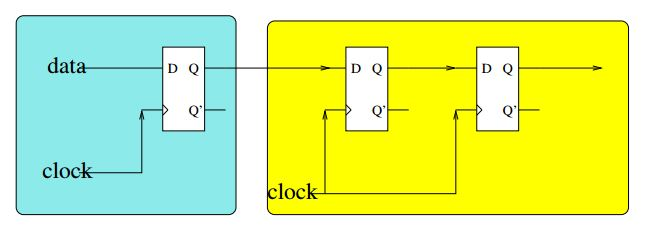
\includegraphics[width=\linewidth]{syncer}
\item Synchronizer doesn't provide a guarantee of metastability but reduces its likelihood. There must be a trade off between an acceptable probability of failure and speed/power consumption of the synchronizer.
\item GALS - Globally Asynchronous Locally Synchronous. (As it says on the tin).
\end{itemize}
\end{document}






















